\chapter{Task2}
\section{a)}
If we chose the machine $M$ as follows: $$M = (q_0, \emptyset, \delta, q_0, {q_0})$$
Then it can be proved that the only language accepted by a machine which has only the start state is the empty string $\epsilon$. 
So the second machine would have as complement language $$\Sigma^* \backslash \epsilon \rightarrow \epsilon \backslash \epsilon = \emptyset$$ remembering that $\emptyset^* = \epsilon$.\\
 So this would mean that the machine $M'$ would be something similar to this. 
\begin{center}
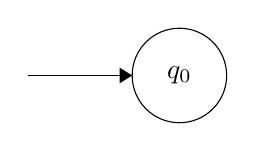
\begin{tikzpicture}[scale=0.2]
\tikzstyle{every node}+=[inner sep=0pt]
\draw [black] (25.5,-26.5) circle (3);
\draw (25.5,-26.5) node {$q_0$};
\draw [black] (15.9,-26.5) -- (22.5,-26.5);
\fill [black] (22.5,-26.5) -- (21.7,-26) -- (21.7,-27);
\end{tikzpicture}
\end{center}
Thus meaning that no language could be accepted by this machine.
\section{b)}
\newpage
\section{c)}
\begin{center}
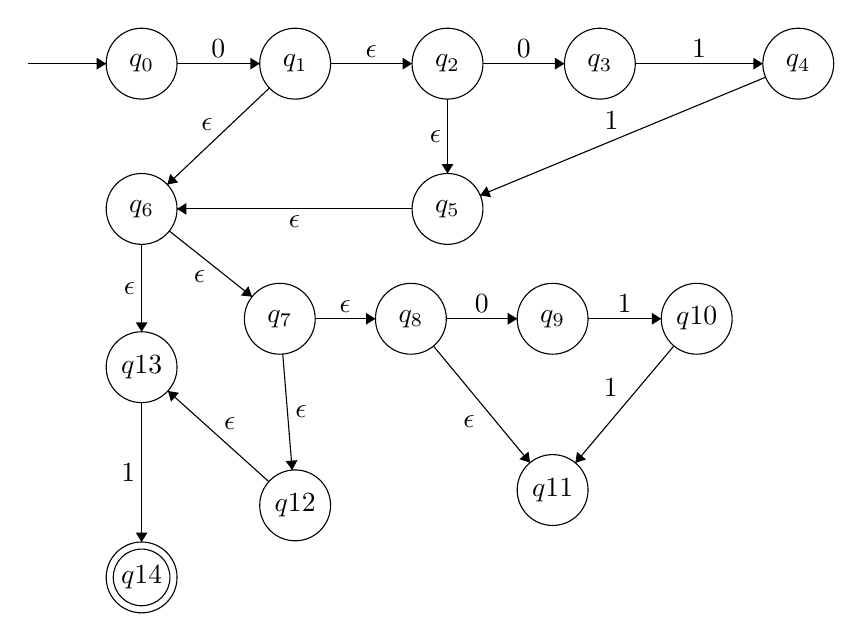
\begin{tikzpicture}[scale=0.15]
\tikzstyle{every node}+=[inner sep=0pt]
\draw [black] (9.7,-7.4) circle (3);
\draw (9.7,-7.4) node {$q_0$};
\draw [black] (22.7,-7.4) circle (3);
\draw (22.7,-7.4) node {$q_1$};
\draw [black] (35.6,-7.4) circle (3);
\draw (35.6,-7.4) node {$q_2$};
\draw [black] (48.5,-7.4) circle (3);
\draw (48.5,-7.4) node {$q_3$};
\draw [black] (65.3,-7.4) circle (3);
\draw (65.3,-7.4) node {$q_4$};
\draw [black] (35.6,-19.7) circle (3);
\draw (35.6,-19.7) node {$q_5$};
\draw [black] (9.7,-19.7) circle (3);
\draw (9.7,-19.7) node {$q_6$};
\draw [black] (21.4,-29) circle (3);
\draw (21.4,-29) node {$q_7$};
\draw [black] (32.5,-29) circle (3);
\draw (32.5,-29) node {$q_8$};
\draw [black] (44.5,-29) circle (3);
\draw (44.5,-29) node {$q_9$};
\draw [black] (56.7,-29) circle (3);
\draw (56.7,-29) node {$q10$};
\draw [black] (44.5,-43.5) circle (3);
\draw (44.5,-43.5) node {$q11$};
\draw [black] (22.7,-44.8) circle (3);
\draw (22.7,-44.8) node {$q12$};
\draw [black] (9.7,-33.1) circle (3);
\draw (9.7,-33.1) node {$q13$};
\draw [black] (9.7,-50.9) circle (3);
\draw (9.7,-50.9) node {$q14$};
\draw [black] (9.7,-50.9) circle (2.4);
\draw [black] (0.1,-7.4) -- (6.7,-7.4);
\fill [black] (6.7,-7.4) -- (5.9,-6.9) -- (5.9,-7.9);
\draw [black] (12.7,-7.4) -- (19.7,-7.4);
\fill [black] (19.7,-7.4) -- (18.9,-6.9) -- (18.9,-7.9);
\draw (16.2,-6.9) node [above] {$0$};
\draw [black] (20.52,-9.46) -- (11.88,-17.64);
\fill [black] (11.88,-17.64) -- (12.8,-17.45) -- (12.12,-16.73);
\draw (15.24,-13.07) node [above] {$\epsilon$};
\draw [black] (25.7,-7.4) -- (32.6,-7.4);
\fill [black] (32.6,-7.4) -- (31.8,-6.9) -- (31.8,-7.9);
\draw (29.15,-6.9) node [above] {$\epsilon$};
\draw [black] (38.6,-7.4) -- (45.5,-7.4);
\fill [black] (45.5,-7.4) -- (44.7,-6.9) -- (44.7,-7.9);
\draw (42.05,-6.9) node [above] {$0$};
\draw [black] (35.6,-10.4) -- (35.6,-16.7);
\fill [black] (35.6,-16.7) -- (36.1,-15.9) -- (35.1,-15.9);
\draw (35.1,-13.55) node [left] {$\epsilon$};
\draw [black] (51.5,-7.4) -- (62.3,-7.4);
\fill [black] (62.3,-7.4) -- (61.5,-6.9) -- (61.5,-7.9);
\draw (56.9,-6.9) node [above] {$1$};
\draw [black] (62.53,-8.55) -- (38.37,-18.55);
\fill [black] (38.37,-18.55) -- (39.3,-18.71) -- (38.92,-17.78);
\draw (49.49,-13.04) node [above] {$1$};
\draw [black] (32.6,-19.7) -- (12.7,-19.7);
\fill [black] (12.7,-19.7) -- (13.5,-20.2) -- (13.5,-19.2);
\draw (22.65,-20.2) node [below] {$\epsilon$};
\draw [black] (9.7,-22.7) -- (9.7,-30.1);
\fill [black] (9.7,-30.1) -- (10.2,-29.3) -- (9.2,-29.3);
\draw (9.2,-26.4) node [left] {$\epsilon$};
\draw [black] (9.7,-36.1) -- (9.7,-47.9);
\fill [black] (9.7,-47.9) -- (10.2,-47.1) -- (9.2,-47.1);
\draw (9.2,-42) node [left] {$1$};
\draw [black] (12.05,-21.57) -- (19.05,-27.13);
\fill [black] (19.05,-27.13) -- (18.74,-26.24) -- (18.11,-27.03);
\draw (14.6,-24.84) node [below] {$\epsilon$};
\draw [black] (24.4,-29) -- (29.5,-29);
\fill [black] (29.5,-29) -- (28.7,-28.5) -- (28.7,-29.5);
\draw (26.95,-28.5) node [above] {$\epsilon$};
\draw [black] (21.65,-31.99) -- (22.45,-41.81);
\fill [black] (22.45,-41.81) -- (22.89,-40.97) -- (21.89,-41.05);
\draw (22.67,-36.84) node [right] {$\epsilon$};
\draw [black] (35.5,-29) -- (41.5,-29);
\fill [black] (41.5,-29) -- (40.7,-28.5) -- (40.7,-29.5);
\draw (38.5,-28.5) node [above] {$0$};
\draw [black] (47.5,-29) -- (53.7,-29);
\fill [black] (53.7,-29) -- (52.9,-28.5) -- (52.9,-29.5);
\draw (50.6,-28.5) node [above] {$1$};
\draw [black] (54.77,-31.3) -- (46.43,-41.2);
\fill [black] (46.43,-41.2) -- (47.33,-40.91) -- (46.56,-40.27);
\draw (50.05,-34.81) node [left] {$1$};
\draw [black] (34.41,-31.31) -- (42.59,-41.19);
\fill [black] (42.59,-41.19) -- (42.46,-40.25) -- (41.69,-40.89);
\draw (37.95,-37.68) node [left] {$\epsilon$};
\draw [black] (20.47,-42.79) -- (11.93,-35.11);
\fill [black] (11.93,-35.11) -- (12.19,-36.01) -- (12.86,-35.27);
\draw (17.16,-38.46) node [above] {$\epsilon$};
\end{tikzpicture}
\end{center}
